\documentclass[aps,prl,reprint]{revtex4-2}

\usepackage{amsmath}
\usepackage{amssymb}
\usepackage{graphicx}
\usepackage{bm}
\usepackage{hyperref}
\usepackage{fancyhdr}

\pagestyle{fancy}
\fancyhf{}
\fancyhead[C]{\small Preprint -- Work in Progress}
\fancyfoot[R]{\small QuantumToy TRF preprint v0.2}
\renewcommand{\headrulewidth}{0pt}

\begin{document}

\title{Thick Reality Front: a numerical framework for spacetime structure in quantum evolution}

\author{Saku H\"am\"al\"ainen}

\date{\today}

\begin{abstract}

We introduce a computational framework for exploring a
``thick reality front'' (TRF) description of quantum dynamics.
Instead of associating physical structure with a single
instantaneous wavefunction, the framework assumes that observable
patterns may emerge from a finite temporal region surrounding
the present.

Forward quantum evolution from preparation is combined with
backward propagation conditioned on detection events.
Their local amplitude overlap produces a spacetime field that
highlights regions simultaneously compatible with preparation
and measurement.

Numerical simulations of a double-slit experiment demonstrate
that this overlap field often develops coherent ridge structures
that trace narrow probability flow channels through spacetime.

Baseline simulations without the thick-front operator are also
presented for comparison, allowing the influence of the TRF
framework on branch structure and ridge stability to be examined.

The framework reproduces standard quantum predictions while
providing a geometric visualization of probability flow between
preparation and measurement.

\end{abstract}

\maketitle


\section{Introduction}

Quantum mechanics describes the evolution of a system through the
Schr\"odinger equation

\begin{equation}
i\hbar \partial_t \psi = H\psi .
\end{equation}

While the equation determines the unitary evolution of the
wavefunction, measurement outcomes appear to select definite
results from a superposition of possibilities.

Several approaches attempt to address this issue, including
collapse models, Bohmian mechanics, and time-symmetric
formulations of quantum theory. Time-symmetric approaches
suggest that both preparation and measurement conditions may
play roles in shaping the structure of quantum processes.

In this work we explore a computational framework inspired by
this idea. Rather than associating physical structure with a
single time slice of the wavefunction, we assume that observable
structure may emerge from a finite temporal region surrounding
the present. We refer to this region as a \textit{thick reality
front}.

\begin{figure}[t]
\centering
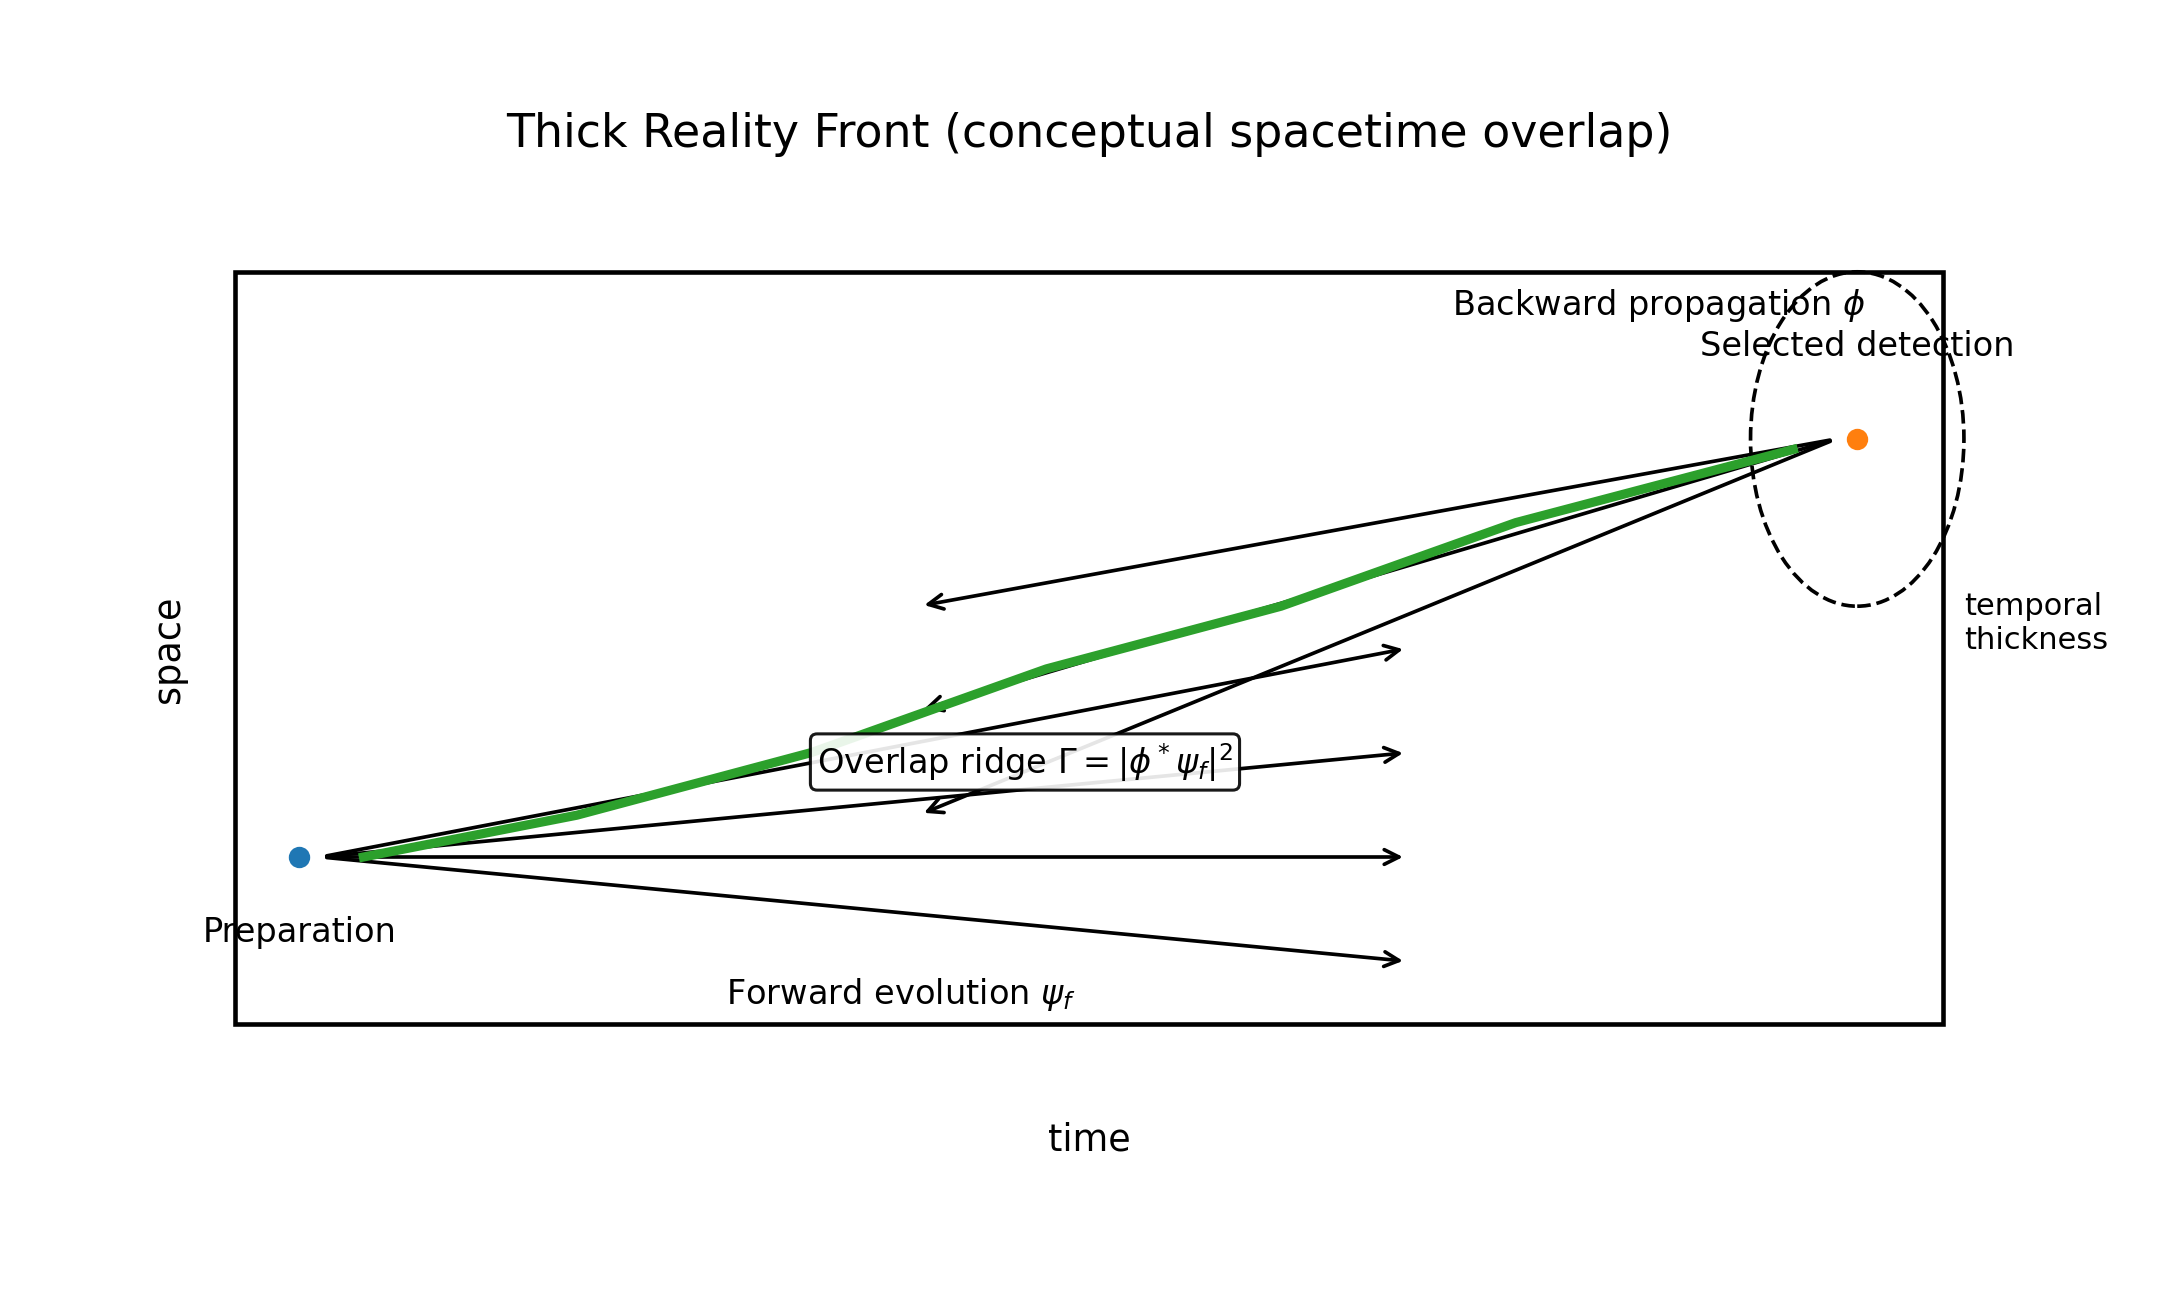
\includegraphics[width=\linewidth]{trf_concept_clean_v02.png}
\caption{
Conceptual illustration of the thick reality front (TRF).
Forward evolution from the preparation event produces a
spreading wavefunction $\psi_f$.
Backward propagation from a selected detection event produces
a retrodictive wave $\phi$.
Their local amplitude overlap
$\Gamma = |\phi^*\psi_f|^2$ highlights spacetime regions
supported simultaneously by both conditions.
}
\end{figure}

The purpose of this work is not to propose a new fundamental
dynamical law but to develop a numerical framework for analyzing
forward–backward amplitude structures and the spacetime patterns
that emerge from them.



\section{Baseline quantum evolution}

Before introducing the TRF framework it is useful to examine the
baseline quantum dynamics.

Forward evolution from an initial state $\psi_0$ is given by

\begin{equation}
\psi_f(t) = U(t,t_0)\psi_0 .
\end{equation}

The corresponding probability density is

\begin{equation}
\rho_f(x,t) = |\psi_f(x,t)|^2 .
\end{equation}

In numerical simulations of a double-slit geometry this
forward evolution produces the familiar interference pattern
on a downstream detection screen.

The baseline dynamics may already exhibit structured probability
flow patterns upstream of the detection screen.
Understanding these structures provides an important reference
for evaluating the additional effects introduced by the
thick-front framework.



\section{Forward and backward evolution}

Suppose a detection occurs at position $x_d$ and time $t_d$.

We construct a localized detection state

\begin{equation}
\phi(x,t_d) =
\exp\!\left(
-\frac{(x-x_d)^2}{2\sigma_c^2}
\right).
\end{equation}

Backward propagation is defined through the adjoint evolution

\begin{equation}
\phi(t) = U^\dagger(t_d,t)\phi(t_d).
\end{equation}

The forward and backward states can therefore be defined at
every intermediate spacetime point.



\section{Amplitude overlap field}

The central quantity in the TRF framework is the local amplitude
overlap

\begin{equation}
A(x,t) = \phi^*(x,t)\psi_f(x,t).
\end{equation}

The ridge intensity field is then defined as

\begin{equation}
\Gamma(x,t) = |A(x,t)|^2 .
\end{equation}

Large values of $\Gamma$ identify spacetime regions that are
simultaneously compatible with both preparation and measurement
conditions.

In numerical experiments this field frequently develops narrow
high-intensity structures forming continuous paths through
spacetime.



\section{Temporal thickness}

Instead of using a single detection time we allow a temporal
distribution of possible detection times within a window of
width $\sigma_T$.

Backward states are therefore averaged as

\begin{equation}
E_{\mathrm{mix}}(x,t)
=
\sum_k
w_k
|\phi_k(x,t)|^2 ,
\end{equation}

with Gaussian weights

\begin{equation}
w_k =
\frac{
\exp[-(t_k-t_d)^2/(2\sigma_T^2)]
}{
\sum_j
\exp[-(t_j-t_d)^2/(2\sigma_T^2)]
}.
\end{equation}

This produces a temporally extended retrodictive weighting
representing the finite thickness of the reality front.



\section{Ridge extraction}

The overlap field $\Gamma(x,t)$ often develops narrow
high-intensity structures.

The simplest ridge trajectory is defined by

\begin{equation}
\mathbf r_R(t)
=
\operatorname*{arg\,max}_{\mathbf r}
\Gamma(\mathbf r,t).
\end{equation}

More stable ridge definitions include centroid estimation
within the top intensity fraction, snapping to nearby local
maxima, and local maximum tracking across frames.

These methods improve temporal continuity when multiple
competing maxima are present.



\section{Velocity field comparison}

The quantum probability current is

\begin{equation}
\mathbf j =
\frac{\hbar}{m}
\mathrm{Im}
(\psi^* \nabla \psi).
\end{equation}

This defines the velocity field

\begin{equation}
\mathbf v = \frac{\mathbf j}{\rho_f}.
\end{equation}

Bohmian trajectories constructed from this velocity field
provide a useful comparison with ridge trajectories extracted
from the overlap field.



\section{Thick-front operator}

The numerical framework can optionally include a
\textit{thick-front operator} that modifies the forward evolution
according to local coherence structure.

The purpose of this operator is not to replace the Schr\"odinger
dynamics but to explore how a finite spacetime thickness of
physical structure might influence branch competition and
ridge formation.

The specific numerical form used in the present simulations
includes

\begin{itemize}

\item local coherence sharpening

\item optional branch competition between nearby maxima

\item normalization preserving overall probability

\end{itemize}

The precise functional form used in the present experiments is
given in Ref.~[placeholder] or the accompanying code repository
\cite{quantumtoy}.



\section{Numerical experiment}

We simulate a two-dimensional double-slit experiment using the
split-operator method.

A Gaussian wave packet propagates toward a barrier containing
two narrow slits and forms an interference pattern on a
downstream screen.

Forward evolution generates the interference pattern while
backward propagation from a selected click state produces a
retrodictive field.

The overlap field $\Gamma$ then highlights spacetime channels
connecting the preparation region with the selected detection
event.



\section{Baseline versus TRF comparison}

To evaluate the influence of the thick-front operator we perform
simulations both with and without this modification.

Baseline simulations reproduce standard Schr\"odinger dynamics.
The TRF simulations introduce the additional coherence-based
operator described above.

Qualitative comparisons focus on

\begin{itemize}

\item ridge sharpness

\item stability of ridge trajectories

\item suppression or enhancement of nearby competing branches

\item agreement with Bohmian trajectory structures

\end{itemize}

Representative results are shown in
Fig.~[placeholder].

In preliminary experiments the TRF framework tends to emphasize
narrow ridge-like probability channels while suppressing some
nearby competing structures.



\section{Limitations}

The present framework is exploratory and several limitations
should be noted.

\begin{itemize}

\item numerical results depend on grid resolution

\item competition operators may introduce discretization artifacts

\item the framework does not yet include a full detector model

\item the thick-front operator is currently phenomenological

\end{itemize}

Future work will investigate more physically motivated
implementations and improved numerical stability.



\section{Conclusion}

We introduced a computational framework for exploring thick
reality front descriptions of quantum dynamics.

By combining forward evolution with backward propagation from
detection events the method produces structured spacetime
overlap fields.

These fields frequently reveal coherent ridge structures that
trace probability flow between preparation and measurement.

Baseline simulations demonstrate that similar structures may
already exist in the underlying quantum dynamics, while the
TRF framework modifies their prominence and stability.

The framework provides a geometric visualization of spacetime
probability structure and may offer a useful tool for exploring
time-symmetric aspects of quantum evolution.



\bibliography{trf_refs}

\end{document}